% Created by tikzDevice version 0.12.6 on 2026-02-03 11:35:31
% !TEX encoding = UTF-8 Unicode
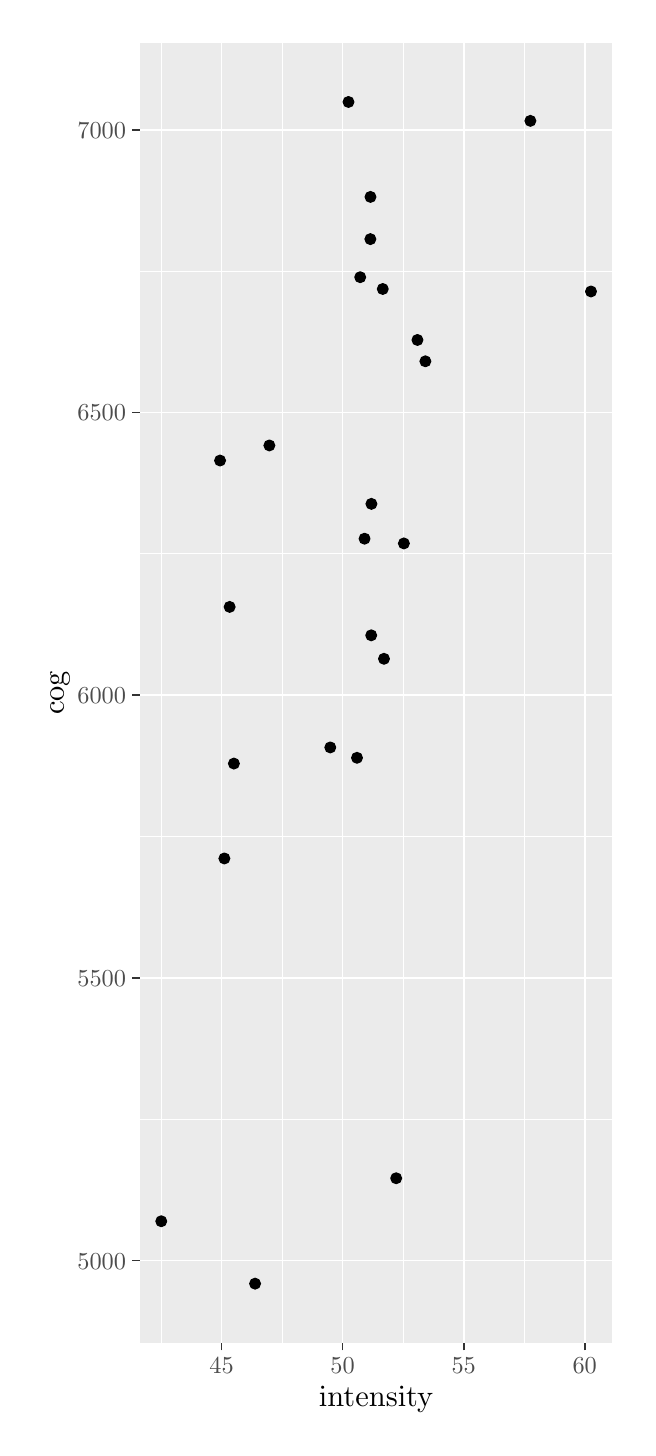
\begin{tikzpicture}[x=1pt,y=1pt]
\definecolor{fillColor}{RGB}{255,255,255}
\path[use as bounding box,fill=fillColor,fill opacity=0.00] (0,0) rectangle (216.81,505.89);
\begin{scope}
\path[clip] (  0.00,  0.00) rectangle (216.81,505.89);
\definecolor{drawColor}{RGB}{255,255,255}
\definecolor{fillColor}{RGB}{255,255,255}

\path[draw=drawColor,line width= 0.6pt,line join=round,line cap=round,fill=fillColor] (  0.00,  0.00) rectangle (216.81,505.89);
\end{scope}
\begin{scope}
\path[clip] ( 40.51, 30.69) rectangle (211.31,500.39);
\definecolor{fillColor}{gray}{0.92}

\path[fill=fillColor] ( 40.51, 30.69) rectangle (211.31,500.39);
\definecolor{drawColor}{RGB}{255,255,255}

\path[draw=drawColor,line width= 0.3pt,line join=round] ( 40.51,111.44) --
	(211.31,111.44);

\path[draw=drawColor,line width= 0.3pt,line join=round] ( 40.51,213.60) --
	(211.31,213.60);

\path[draw=drawColor,line width= 0.3pt,line join=round] ( 40.51,315.76) --
	(211.31,315.76);

\path[draw=drawColor,line width= 0.3pt,line join=round] ( 40.51,417.93) --
	(211.31,417.93);

\path[draw=drawColor,line width= 0.3pt,line join=round] ( 48.21, 30.69) --
	( 48.21,500.39);

\path[draw=drawColor,line width= 0.3pt,line join=round] ( 91.94, 30.69) --
	( 91.94,500.39);

\path[draw=drawColor,line width= 0.3pt,line join=round] (135.68, 30.69) --
	(135.68,500.39);

\path[draw=drawColor,line width= 0.3pt,line join=round] (179.42, 30.69) --
	(179.42,500.39);

\path[draw=drawColor,line width= 0.6pt,line join=round] ( 40.51, 60.36) --
	(211.31, 60.36);

\path[draw=drawColor,line width= 0.6pt,line join=round] ( 40.51,162.52) --
	(211.31,162.52);

\path[draw=drawColor,line width= 0.6pt,line join=round] ( 40.51,264.68) --
	(211.31,264.68);

\path[draw=drawColor,line width= 0.6pt,line join=round] ( 40.51,366.84) --
	(211.31,366.84);

\path[draw=drawColor,line width= 0.6pt,line join=round] ( 40.51,469.01) --
	(211.31,469.01);

\path[draw=drawColor,line width= 0.6pt,line join=round] ( 70.07, 30.69) --
	( 70.07,500.39);

\path[draw=drawColor,line width= 0.6pt,line join=round] (113.81, 30.69) --
	(113.81,500.39);

\path[draw=drawColor,line width= 0.6pt,line join=round] (157.55, 30.69) --
	(157.55,500.39);

\path[draw=drawColor,line width= 0.6pt,line join=round] (201.29, 30.69) --
	(201.29,500.39);
\definecolor{drawColor}{RGB}{0,0,0}
\definecolor{fillColor}{RGB}{0,0,0}

\path[draw=drawColor,line width= 0.4pt,line join=round,line cap=round,fill=fillColor] ( 71.08,205.68) circle (  1.96);

\path[draw=drawColor,line width= 0.4pt,line join=round,line cap=round,fill=fillColor] (121.73,321.23) circle (  1.96);

\path[draw=drawColor,line width= 0.4pt,line join=round,line cap=round,fill=fillColor] (203.55,410.56) circle (  1.96);

\path[draw=drawColor,line width= 0.4pt,line join=round,line cap=round,fill=fillColor] (135.94,319.52) circle (  1.96);

\path[draw=drawColor,line width= 0.4pt,line join=round,line cap=round,fill=fillColor] ( 82.17, 52.04) circle (  1.96);

\path[draw=drawColor,line width= 0.4pt,line join=round,line cap=round,fill=fillColor] ( 74.52,239.97) circle (  1.96);

\path[draw=drawColor,line width= 0.4pt,line join=round,line cap=round,fill=fillColor] (124.14,286.31) circle (  1.96);

\path[draw=drawColor,line width= 0.4pt,line join=round,line cap=round,fill=fillColor] (119.00,242.05) circle (  1.96);

\path[draw=drawColor,line width= 0.4pt,line join=round,line cap=round,fill=fillColor] (123.83,429.48) circle (  1.96);

\path[draw=drawColor,line width= 0.4pt,line join=round,line cap=round,fill=fillColor] (123.87,444.73) circle (  1.96);

\path[draw=drawColor,line width= 0.4pt,line join=round,line cap=round,fill=fillColor] (124.21,333.81) circle (  1.96);

\path[draw=drawColor,line width= 0.4pt,line join=round,line cap=round,fill=fillColor] ( 48.27, 74.59) circle (  1.96);

\path[draw=drawColor,line width= 0.4pt,line join=round,line cap=round,fill=fillColor] (109.35,245.80) circle (  1.96);

\path[draw=drawColor,line width= 0.4pt,line join=round,line cap=round,fill=fillColor] (128.75,277.83) circle (  1.96);

\path[draw=drawColor,line width= 0.4pt,line join=round,line cap=round,fill=fillColor] (140.84,393.04) circle (  1.96);

\path[draw=drawColor,line width= 0.4pt,line join=round,line cap=round,fill=fillColor] (133.16, 90.13) circle (  1.96);

\path[draw=drawColor,line width= 0.4pt,line join=round,line cap=round,fill=fillColor] (115.92,479.04) circle (  1.96);

\path[draw=drawColor,line width= 0.4pt,line join=round,line cap=round,fill=fillColor] (143.71,385.33) circle (  1.96);

\path[draw=drawColor,line width= 0.4pt,line join=round,line cap=round,fill=fillColor] ( 69.52,349.47) circle (  1.96);

\path[draw=drawColor,line width= 0.4pt,line join=round,line cap=round,fill=fillColor] (120.16,415.72) circle (  1.96);

\path[draw=drawColor,line width= 0.4pt,line join=round,line cap=round,fill=fillColor] (128.31,411.46) circle (  1.96);

\path[draw=drawColor,line width= 0.4pt,line join=round,line cap=round,fill=fillColor] (181.65,472.21) circle (  1.96);

\path[draw=drawColor,line width= 0.4pt,line join=round,line cap=round,fill=fillColor] ( 87.34,354.92) circle (  1.96);

\path[draw=drawColor,line width= 0.4pt,line join=round,line cap=round,fill=fillColor] ( 72.98,296.58) circle (  1.96);
\end{scope}
\begin{scope}
\path[clip] (  0.00,  0.00) rectangle (216.81,505.89);
\definecolor{drawColor}{gray}{0.30}

\node[text=drawColor,anchor=base east,inner sep=0pt, outer sep=0pt, scale=  0.88] at ( 35.56, 57.33) {5000};

\node[text=drawColor,anchor=base east,inner sep=0pt, outer sep=0pt, scale=  0.88] at ( 35.56,159.49) {5500};

\node[text=drawColor,anchor=base east,inner sep=0pt, outer sep=0pt, scale=  0.88] at ( 35.56,261.65) {6000};

\node[text=drawColor,anchor=base east,inner sep=0pt, outer sep=0pt, scale=  0.88] at ( 35.56,363.81) {6500};

\node[text=drawColor,anchor=base east,inner sep=0pt, outer sep=0pt, scale=  0.88] at ( 35.56,465.98) {7000};
\end{scope}
\begin{scope}
\path[clip] (  0.00,  0.00) rectangle (216.81,505.89);
\definecolor{drawColor}{gray}{0.20}

\path[draw=drawColor,line width= 0.6pt,line join=round] ( 37.76, 60.36) --
	( 40.51, 60.36);

\path[draw=drawColor,line width= 0.6pt,line join=round] ( 37.76,162.52) --
	( 40.51,162.52);

\path[draw=drawColor,line width= 0.6pt,line join=round] ( 37.76,264.68) --
	( 40.51,264.68);

\path[draw=drawColor,line width= 0.6pt,line join=round] ( 37.76,366.84) --
	( 40.51,366.84);

\path[draw=drawColor,line width= 0.6pt,line join=round] ( 37.76,469.01) --
	( 40.51,469.01);
\end{scope}
\begin{scope}
\path[clip] (  0.00,  0.00) rectangle (216.81,505.89);
\definecolor{drawColor}{gray}{0.20}

\path[draw=drawColor,line width= 0.6pt,line join=round] ( 70.07, 27.94) --
	( 70.07, 30.69);

\path[draw=drawColor,line width= 0.6pt,line join=round] (113.81, 27.94) --
	(113.81, 30.69);

\path[draw=drawColor,line width= 0.6pt,line join=round] (157.55, 27.94) --
	(157.55, 30.69);

\path[draw=drawColor,line width= 0.6pt,line join=round] (201.29, 27.94) --
	(201.29, 30.69);
\end{scope}
\begin{scope}
\path[clip] (  0.00,  0.00) rectangle (216.81,505.89);
\definecolor{drawColor}{gray}{0.30}

\node[text=drawColor,anchor=base,inner sep=0pt, outer sep=0pt, scale=  0.88] at ( 70.07, 19.68) {45};

\node[text=drawColor,anchor=base,inner sep=0pt, outer sep=0pt, scale=  0.88] at (113.81, 19.68) {50};

\node[text=drawColor,anchor=base,inner sep=0pt, outer sep=0pt, scale=  0.88] at (157.55, 19.68) {55};

\node[text=drawColor,anchor=base,inner sep=0pt, outer sep=0pt, scale=  0.88] at (201.29, 19.68) {60};
\end{scope}
\begin{scope}
\path[clip] (  0.00,  0.00) rectangle (216.81,505.89);
\definecolor{drawColor}{RGB}{0,0,0}

\node[text=drawColor,anchor=base,inner sep=0pt, outer sep=0pt, scale=  1.10] at (125.91,  7.64) {intensity};
\end{scope}
\begin{scope}
\path[clip] (  0.00,  0.00) rectangle (216.81,505.89);
\definecolor{drawColor}{RGB}{0,0,0}

\node[text=drawColor,rotate= 90.00,anchor=base,inner sep=0pt, outer sep=0pt, scale=  1.10] at ( 13.08,265.54) {cog};
\end{scope}
\end{tikzpicture}
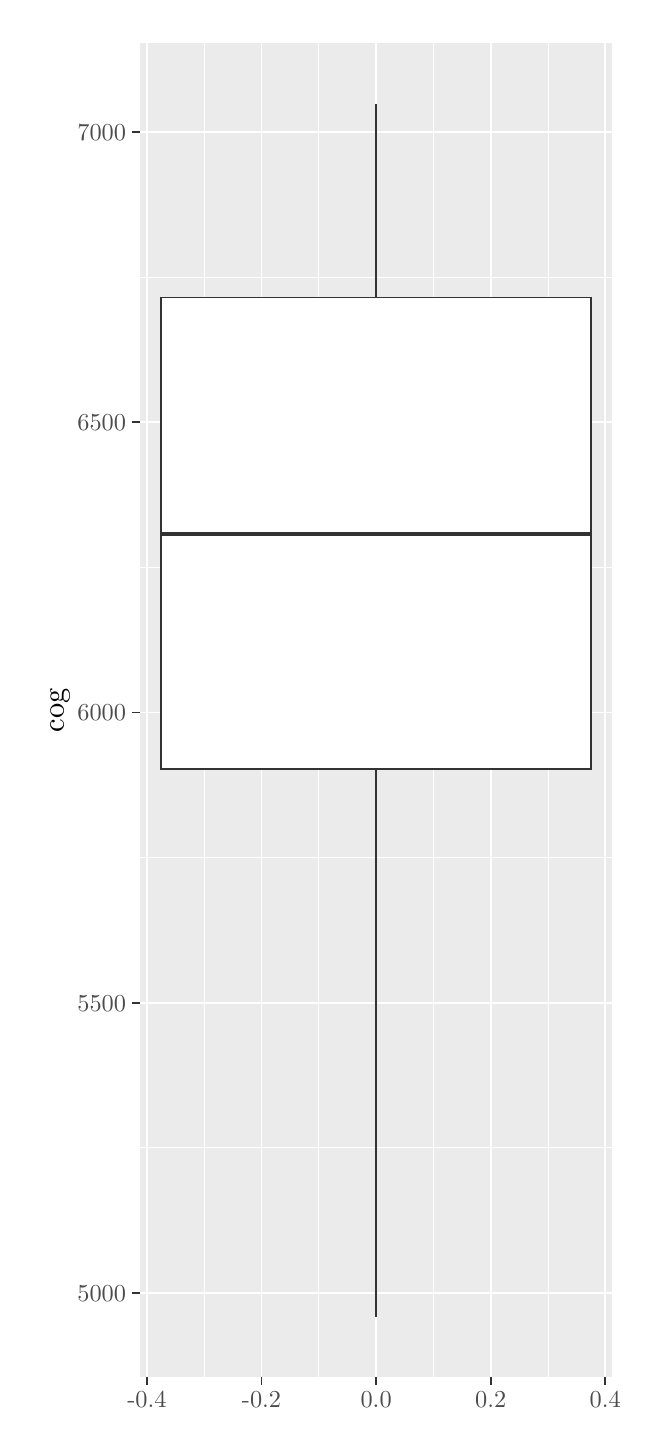
\begin{tikzpicture}[x=1pt,y=1pt]
\definecolor{fillColor}{RGB}{255,255,255}
\path[use as bounding box,fill=fillColor,fill opacity=0.00] (0,0) rectangle (216.81,505.89);
\begin{scope}
\path[clip] (  0.00,  0.00) rectangle (216.81,505.89);
\definecolor{drawColor}{RGB}{255,255,255}
\definecolor{fillColor}{RGB}{255,255,255}

\path[draw=drawColor,line width= 0.6pt,line join=round,line cap=round,fill=fillColor] (  0.00,  0.00) rectangle (216.81,505.89);
\end{scope}
\begin{scope}
\path[clip] ( 40.51, 18.22) rectangle (211.31,500.39);
\definecolor{fillColor}{gray}{0.92}

\path[fill=fillColor] ( 40.51, 18.22) rectangle (211.31,500.39);
\definecolor{drawColor}{RGB}{255,255,255}

\path[draw=drawColor,line width= 0.3pt,line join=round] ( 40.51,101.12) --
	(211.31,101.12);

\path[draw=drawColor,line width= 0.3pt,line join=round] ( 40.51,205.99) --
	(211.31,205.99);

\path[draw=drawColor,line width= 0.3pt,line join=round] ( 40.51,310.86) --
	(211.31,310.86);

\path[draw=drawColor,line width= 0.3pt,line join=round] ( 40.51,415.74) --
	(211.31,415.74);

\path[draw=drawColor,line width= 0.3pt,line join=round] ( 63.80, 18.22) --
	( 63.80,500.39);

\path[draw=drawColor,line width= 0.3pt,line join=round] (105.21, 18.22) --
	(105.21,500.39);

\path[draw=drawColor,line width= 0.3pt,line join=round] (146.61, 18.22) --
	(146.61,500.39);

\path[draw=drawColor,line width= 0.3pt,line join=round] (188.02, 18.22) --
	(188.02,500.39);

\path[draw=drawColor,line width= 0.6pt,line join=round] ( 40.51, 48.68) --
	(211.31, 48.68);

\path[draw=drawColor,line width= 0.6pt,line join=round] ( 40.51,153.56) --
	(211.31,153.56);

\path[draw=drawColor,line width= 0.6pt,line join=round] ( 40.51,258.43) --
	(211.31,258.43);

\path[draw=drawColor,line width= 0.6pt,line join=round] ( 40.51,363.30) --
	(211.31,363.30);

\path[draw=drawColor,line width= 0.6pt,line join=round] ( 40.51,468.17) --
	(211.31,468.17);

\path[draw=drawColor,line width= 0.6pt,line join=round] ( 43.10, 18.22) --
	( 43.10,500.39);

\path[draw=drawColor,line width= 0.6pt,line join=round] ( 84.50, 18.22) --
	( 84.50,500.39);

\path[draw=drawColor,line width= 0.6pt,line join=round] (125.91, 18.22) --
	(125.91,500.39);

\path[draw=drawColor,line width= 0.6pt,line join=round] (167.32, 18.22) --
	(167.32,500.39);

\path[draw=drawColor,line width= 0.6pt,line join=round] (208.72, 18.22) --
	(208.72,500.39);
\definecolor{drawColor}{gray}{0.20}

\path[draw=drawColor,line width= 0.6pt,line join=round] (125.91,408.41) -- (125.91,478.47);

\path[draw=drawColor,line width= 0.6pt,line join=round] (125.91,238.08) -- (125.91, 40.14);
\definecolor{fillColor}{RGB}{255,255,255}

\path[draw=drawColor,line width= 0.6pt,fill=fillColor] ( 48.27,408.41) --
	( 48.27,238.08) --
	(203.55,238.08) --
	(203.55,408.41) --
	( 48.27,408.41) --
	cycle;

\path[draw=drawColor,line width= 1.1pt] ( 48.27,322.93) -- (203.55,322.93);
\end{scope}
\begin{scope}
\path[clip] (  0.00,  0.00) rectangle (216.81,505.89);
\definecolor{drawColor}{gray}{0.30}

\node[text=drawColor,anchor=base east,inner sep=0pt, outer sep=0pt, scale=  0.88] at ( 35.56, 45.65) {5000};

\node[text=drawColor,anchor=base east,inner sep=0pt, outer sep=0pt, scale=  0.88] at ( 35.56,150.53) {5500};

\node[text=drawColor,anchor=base east,inner sep=0pt, outer sep=0pt, scale=  0.88] at ( 35.56,255.40) {6000};

\node[text=drawColor,anchor=base east,inner sep=0pt, outer sep=0pt, scale=  0.88] at ( 35.56,360.27) {6500};

\node[text=drawColor,anchor=base east,inner sep=0pt, outer sep=0pt, scale=  0.88] at ( 35.56,465.14) {7000};
\end{scope}
\begin{scope}
\path[clip] (  0.00,  0.00) rectangle (216.81,505.89);
\definecolor{drawColor}{gray}{0.20}

\path[draw=drawColor,line width= 0.6pt,line join=round] ( 37.76, 48.68) --
	( 40.51, 48.68);

\path[draw=drawColor,line width= 0.6pt,line join=round] ( 37.76,153.56) --
	( 40.51,153.56);

\path[draw=drawColor,line width= 0.6pt,line join=round] ( 37.76,258.43) --
	( 40.51,258.43);

\path[draw=drawColor,line width= 0.6pt,line join=round] ( 37.76,363.30) --
	( 40.51,363.30);

\path[draw=drawColor,line width= 0.6pt,line join=round] ( 37.76,468.17) --
	( 40.51,468.17);
\end{scope}
\begin{scope}
\path[clip] (  0.00,  0.00) rectangle (216.81,505.89);
\definecolor{drawColor}{gray}{0.20}

\path[draw=drawColor,line width= 0.6pt,line join=round] ( 43.10, 15.47) --
	( 43.10, 18.22);

\path[draw=drawColor,line width= 0.6pt,line join=round] ( 84.50, 15.47) --
	( 84.50, 18.22);

\path[draw=drawColor,line width= 0.6pt,line join=round] (125.91, 15.47) --
	(125.91, 18.22);

\path[draw=drawColor,line width= 0.6pt,line join=round] (167.32, 15.47) --
	(167.32, 18.22);

\path[draw=drawColor,line width= 0.6pt,line join=round] (208.72, 15.47) --
	(208.72, 18.22);
\end{scope}
\begin{scope}
\path[clip] (  0.00,  0.00) rectangle (216.81,505.89);
\definecolor{drawColor}{gray}{0.30}

\node[text=drawColor,anchor=base,inner sep=0pt, outer sep=0pt, scale=  0.88] at ( 43.10,  7.21) {-0.4};

\node[text=drawColor,anchor=base,inner sep=0pt, outer sep=0pt, scale=  0.88] at ( 84.50,  7.21) {-0.2};

\node[text=drawColor,anchor=base,inner sep=0pt, outer sep=0pt, scale=  0.88] at (125.91,  7.21) {0.0};

\node[text=drawColor,anchor=base,inner sep=0pt, outer sep=0pt, scale=  0.88] at (167.32,  7.21) {0.2};

\node[text=drawColor,anchor=base,inner sep=0pt, outer sep=0pt, scale=  0.88] at (208.72,  7.21) {0.4};
\end{scope}
\begin{scope}
\path[clip] (  0.00,  0.00) rectangle (216.81,505.89);
\definecolor{drawColor}{RGB}{0,0,0}

\node[text=drawColor,rotate= 90.00,anchor=base,inner sep=0pt, outer sep=0pt, scale=  1.10] at ( 13.08,259.31) {cog};
\end{scope}
\end{tikzpicture}
